%
%  untitled
%
%  Created by Sam Anzaroot on 2012-10-05.
%  Copyright (c) 2012 __MyCompanyName__. All rights reserved.
%
\documentclass[twocolumn,letterpaper]{article}

% Use utf-8 encoding for foreign characters
\usepackage[utf8]{inputenc}

% Setup for fullpage use
\usepackage{fullpage}
\usepackage{subfigure}

% Multipart figures
%\usepackage{subfigure}

% More symbols
\usepackage{amsmath}

% Package for including code in the document
\usepackage{listings}

\usepackage{ifpdf}

\ifpdf
\usepackage[pdftex]{graphicx}
\else
\usepackage{graphicx}
\fi

\usepackage{todonotes}

\setlength{\marginparwidth}{2cm}

\title{Author Linkage in Records using Temporal Information and Conditional Random Fields}
\author{Sam Anzaroot, Jiaping Zheng}

\date{}

\begin{document}

\ifpdf
\DeclareGraphicsExtensions{.pdf, .jpg, .tif}
\else
\DeclareGraphicsExtensions{.eps, .jpg}
\fi

\maketitle

\section{Introduction} % (fold)
\label{sec:introduction}
Record Linking is the task of clustering records in a database such that elements in the same cluster refer to the same real world object. For example, in the DBLP page for David Smith, the first three publications are authored by three different individuals.  In fact, among the 37 publications listed under this name, there are 21 authors.  The output of a record linker would cluster each David Smith's publications into separate clusters. Various attempts have been made for record linking authors of publications listed in datasets such as DBLP. This task is important because there are many downstream applications that require clean clustering of such information, for example, determining the most prolific authors is only accurate if such clusterings are valid. Network analysis of coauthorship also depends on correct clustering of authors. In this report, we define strings of author names as author mentions, and clusters of author mentions referring to the same person as entities. The goal of the task is to cluster all mentions into the appropriate entities. This task requires a classifier to determine the matchings between two mentions. This task is not a solved one, and we will attempt to build a more robust classifier.
% section introduction (end)

\section{Related Work} % (fold)
\label{sec:related_work}
\paragraph{Survey of Related work} % (fold)
\label{par:survey_of_related_work}
The research field of record clustering is a very active one. This task is important for many different applications, and as such there are many different names for this task, including record clustering, record deduplication, record linking, entity resolution, etc. There are many components to a record linking system. The first are methods of paring down which records are in need of clustering for efficiency, called blocking methods. The task also requires a system for classifying whether or not a set of records match. In addition, methods of effectively clustering supersets of records independently classified are necessary. In order to classify records, effective similarity and/or compatibility measures are needed as features in a classifier. In this report, we are focusing in on building a better classifier for disambiguating authors in DBLP, and generating better features.
% paragraph survey_of_related_work (end)

Similarity metrics are important for classification as they provide information in which a classifier can make a decision on. Others have shown that adding temporal information into metrics can enhance the quality of classification \cite{DBLP:journals/fcsc/LiDMS12}. These metrics are weighted by how relevant the metrics are given the distance in time between the two records. This weighting is learned from a set of annotated data.

Various numbers of people have attempted to build classifiers using graphical models that include complex dependencies. For example, ``Multi-Relational Record Linkage'' \cite{Domingos04multi} models the record linking problem as a conditional random field which improved F1 performance on a publication deduplication task. In this CRF model, each pair of publication records has a binary latent variable to model whether the records are duplicates.  The observations are modeled using similarity functions.  ``Information nodes'' connect the binary duplication variables and the observation nodes which represent whether the fields of the publication in two records match.

``A Conditional Model of Deduplication for Multi-Type Relational Data'' \cite{Culotta05aconditional} extends the model previously stated by making the ``information nodes'' first-class variables in the model.  Binary latent variables that indicate record duplication (both paper and venue) are connected in the CRF to capture the interdependencies between the deduplication results of publications and venues.  For example, equivalent venue records that are merged should result in weights in CRF that also encourage merging of paper records.  To perform inference of finding optimal configurations of the latent variables, the authors convert the model into a weighted undirected graph to find an optimal partitioning.  Learning is approximated by maximizing the product of local marginals using limited-memory BFGS.  Their experiments show an up to a 30\% error reduction in venue deduplication and 20\% in paper deduplication.
% section related_work (end)

\section{Annotation} % (fold)
\label{sec:annotation}
There is no publicly available resource that we can use to train and test our model.  Thus, we selected 13 highly ambiguous names (including for example, John Smith and Wang Chen) from the DBLP dataset, and annotated the true clusters.  The annotated dataset contains 715 publications from 193 authors.

To illustrate the difficulty of the problem, we provide a few examples in Table \ref{tbl:examples}.  Notice that the ``Wei Chen'' pair of papers are both about visualization software tools in bioinformatics.  The two journals are also very closely related.  Although the authors' affiliations are different, given that the two papers are published 4 year apart, it is reasonable to assume that they are published by the same author who moved between institutions.  However, this turned out to be not the case.  In the second example of ``Wang Chen'', considering their author affiliations are different (the physical locations are far apart) and they are published in the same year, it's reasonable to assume that they are different, especially since this name is a highly common and ambiguous in China.  Looking at the coauthors of the paper, and their affiliations, however, it is more likely that they are the same person, probably with multiple affiliations.
\begin{table*}
  \centering
  \begin{tabular}{l|p{4cm}|l|l|p{4cm}}
    Author & Paper Title  & Venue & Year & Affiliation \\ \hline
    Wei Chen & CGHPRO --- A comprehensive data analysis tool for array CGH & BMC Bioinformatics & 2005 & Max-Planck Institute for Molecular Genetics \\
    Wei Chen & GWAS GUI: graphical browser for the results of whole-genome association studies with high-dimensional phenotypes & Bioinformatics & 2009 & University of Michigan \\ \hline
    Wang Chen & An Artificial Bee Colony with Random Key for Resource-Constrained Project Scheduling & LSMS/ICSEE & 2010 & China North Vehicle Research Institute \\
    Wang Chen & An efficient hybrid algorithm for resource-constrained project scheduling & Inf. Sci. & 2010 & Dalian University of Technology
  \end{tabular}
  \caption{Examples of annotations.}
  \label{tbl:examples}
\end{table*}

We also manually filled in missing author affiliation information from the paper for our affiliation similarity features.  The affiliation information is a highly indicative feature.  However, it is not easy to automatically collect.  Different journals and conferences have different formatting standards.  It is also sometimes embedded in a short biographical text.  Online academic publication repositories such as ACM and IEEE often contain errors in their extracted affiliation information.  When the actual publication is not available to download, it is even harder to annotate its authors' affiliations.  We had to rely on other sources, such as the author's home page or CV.  For example, one paper by John B. Smith published in 1974 is listed in DBLP, but the paper is not available online.  To determine his affiliation at the time of publication, we searched the other more recent publications on his DBLP page to find out his home page.  This 1974 paper was listed in his CV, through which we could determine his affiliation.

% section annotation (end)

\section{Methodology} % (fold)
\label{sec:methodology}
We model the author linkage problem in a conditional random field.

Conditional random fields (CRFs) are undirected graphical models that encode the conditional probability of a set of unobserved random variables $Y$ given a set of observed variables $X$.  Usually the probability can be factored using independence assumptions.  The model can be represented in a graph $G$, where the vertices correspond to the variables $X$ and $Y$.  A potential function $\phi_c$ is defined for every clique $c$ in the graph.  The conditional probability $p(y|x)$ can be expressed as
$$p(y|x)=\frac{1}{Z}\prod_c \phi_c(x_c,y_c),$$
where $Z=\sum_y\prod_c \phi_c(x_c,y_c)$ is a normalization factor.  We assume $\phi_c$ is a log-linear combination of feature functions of the variables in clique $c$, thus
$$\phi_c(x_c,y_c)=\exp\left(\sum_k \lambda_k f_k(x_c,y_c)\right).$$

The model parameters $\{\lambda_k\}$ are learned from training data by
maximum likelihood estimation.  In a CRF model, the log likelihood
function is optimized using numerical optimization methods, such as
limited-memory BFGS or conjugate gradient method. We used the SampleRank algorithm to train our model.
SampleRank is a supervised learning algorithm which works by iterating over each training variable in turn, sampling output proposals from the set of possible values for the variable  \cite{wick2009samplerank}. During each iteration, the SampleRank algorithm updates the weights of the model to match the ranking of an objective function. In our case, we use a 0-1 objective.

Inference corresponds to finding the optimal assignments to the $Y$
variables such that $p(y|x)$ is maximized.  Belief propagation is an exact inference algorithm on tree-structured models.  Approximate algorithms on models with cycles include loopy belief propagation and
MCMC methods. We used MCMC methods for inference in our model.



Specifically, our CRF structure models the conditional probability of
two author mentions referring to the same entity given the publication
information.  The unobserved random variables in our model include one
binary variable for each pair of author mentions that indicates
whether they refer to the same person.  We also define latent random
variables that represent the compatibility between the names of the
authors, between the publication venues, between their affiliations,
and between their coauthors.  The observed variables are similarity
features between author names, venues, affiliations, and coauthors.
The model is shown in Figure \ref{fig:crf}.

\begin{figure*}
\centering
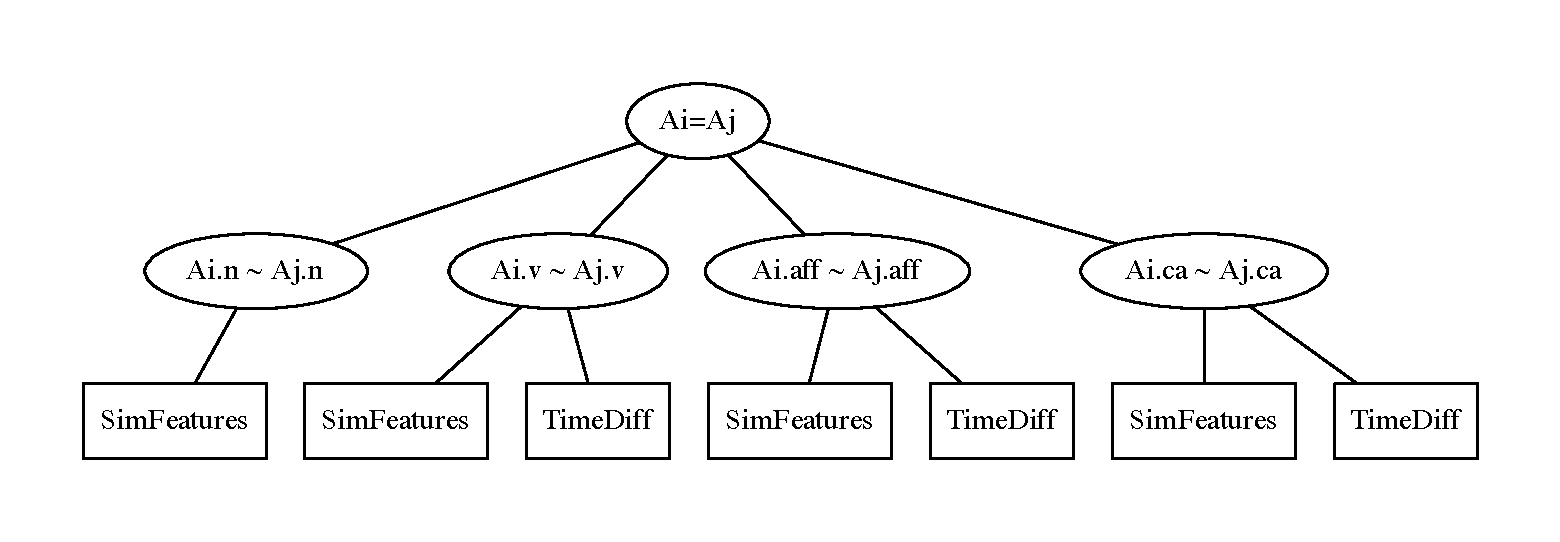
\includegraphics[width=\textwidth]{crf}
\caption{Our CRF model for the author linkage problem.  $A_i$ denotes
  the $i$th author string.  $A_i.n$, $A_i.v$, $A_i.aff$, and $A_i.ca$
  denote the name, venue, affiliation, and coauthors of $A_i$.  The
  oval nodes are unobserved random variables, and the box-shaped ones
  are observed variables.}
\label{fig:crf}
\end{figure*}

\begin{figure}
\centering
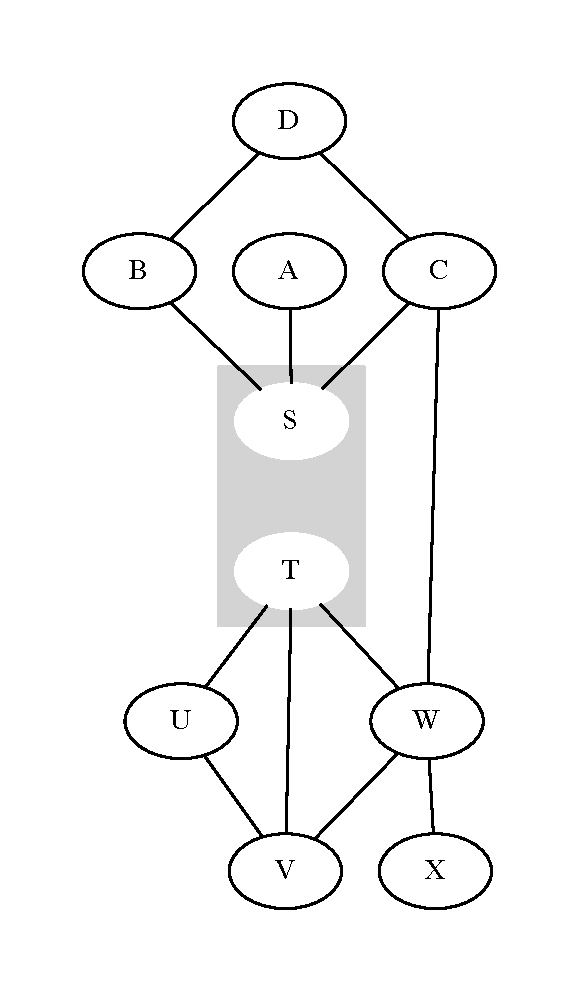
\includegraphics[height=.32\textheight]{coauthor}
\caption{A coauthorship network.  The nodes represent author strings
  in the database.  An edge between two nodes means that the two
  authors coauthored a paper.  $S$ and $T$ are the two author mentions
  that the model is classifying. Edges between $S$, $T$ and other
  nodes mean that the other node is a coauthor mention in the
  publication containing the mentions $S$ and $T$.}
\label{fig:coauthor}
\end{figure}

Unlike the model proposed in Culotta and McCallum
\cite{Culotta05aconditional}, which deduplicates publication title and
venues jointly, our model focuses on author coreference resolution.
Learning and inference in such a complicated model is intractable.
However, since the DBLP data is generated directly from entire
conference proceedings and journals, the publication records are less
noisy.  Our model takes advantage of the reliability of the source
data and deduplicates only ambiguous author information.  Therefore,
our model is more scalable.

Linking pairs of author names is only the first step in the author
linkage problem.  To generate clusters of author mentions that refer
to the same person, we take the transitive closure of the pairwise
predictions from the CRF model.

Since we are comparing pairs of author mentions, it's impractical to
consider all the $O(n^2)$ pairs in the dataset.  We'll also be wasting
effort because most of the pairs clearly do not refer to the same
author.  We follow the method in \cite{McCallum00} to first cluster
the author strings into ``canopies'' and only compare pairs within the
same canopy.  Canopies are soft clusters that can have overlapping
author mentions.  This approach can significantly reduce the number of
pairs we need to compare, and the soft nature of the clusters help
mitigate the problem that the clustering algorithm may have
inaccurately partitioned the data set.  Our canopies are defined as
author mentions that have the same first and last name.

\paragraph{Similarity Features} % (fold)
\label{par:similarity_features}
In order to perform classification we will make use of various similarity and compatibility metrics. One useful metric is string similarity. Simple Levenstein edit distance often works poorly in many of the applications in this domain such as name comparison, since names are often represented in different formats, with the ordering switched, abbreviated etc. Hybrid methods, which combine string-edit distance with token based methods, often are the best performing distance metric in similar tasks \cite{cohen2003comparison}. One such metric is SoftTFIDF. SoftTFIDF works like TFIDF, but on similar tokens instead of just matching tokens. It uses the Jaro-Winkler metric as the similarity metric for tokens. 

The Jaro similarity metric for $s$ and $t$ given $s= s_1,s_2,s_3...,s_i$ and $t= t_1,t_2,t_3...,t_j$ defines a match of $s_i$ to a character $t_j$ if $s_i=t_j$ and j is $\frac{min(s,t)}{2} < |i-j|$. Define $s'$ as the characters that match in $s$ and $t'$ as the characters that match in t. Additionally, define $T$ as half the number of elements that are not exactly matched in position and character in $s$ and in $t$ and $P$ as the maximum of the longest common prefix of $s$ and $t$ or 4. Jaro is then defined as:
\begin{center}
\[
	JARO(s,t) = \frac{1}{3}\left(\frac{|s'|}{|s|}+\frac{|t'|}{|t|}+\frac{|s'|-T}{|s'|}\right)
\]
\end{center}

and Jaro-Winkler is defined as:
\begin{center}
\[
	Jaro-Winkler(s,t) = JARO(s,t) + \frac{P}{10}(1-JARO(s,t))
\]
\end{center}

For SoftTFIDF we need a function $CLOSE(\theta; s; s)$ which is defined as the set of words such that there is some $v \in t$ in which $dist(w; v) > \theta$. SoftTFIDF modifies regular cosine similarity by summing over all words in $CLOSE(\theta; s; t)$ the product of regular TFIDF of $s_w$, $t_w$, and $dist(w;t)$. Jaro-Winkler SoftTFIDF is implemented by using Jaro-Winkler as the distance function.

Affiliation similarity features can be derived from these string similarity functions. For other fields, more involved similarity features are necessary. Such fields include publication name, venue compatibility, and coauthorship compatibility.  For coauthorship compatibility we make use of coauthorship graphs. An example coauthorship graph is displayed in Figure \ref{fig:coauthor}. Given an undirected graph $G=(N \cup M,E)$ where $M$ are the entity mentions of a publication, $N$ are the entities assumed to be correctly disambiguated based on identical string name, each $e \in E$ implies coauthorship between the entities. The edges between the mentions being classified are coauthor mentions in the publication. There cannot be any edges between the two mentions. Our goal with this similarity metric is to determine the connectiveness of the two publication's coauthors. We determine this score by counting how many entities can be reached from in a depth first search initialized from each mention node seperatly. People with ambigious names can potentialy causes erronous linking between two authors who have coauthored papers with two different people with the same name. We try to limit this even from happening by not linking authors who have over 200 coauthors in the DBLP database. If $a$ is the number of coauthors of the first publication, $b$ is the number of coauthors of the second publication, and $c$ is the number of entities reachable from both mentions, our connected score is $\frac{min(c,max(a,b))}{max(a,b)}$. One example graph with only contributing entities shown can be seen in figure \ref{fig:chen}.

\begin{figure*}
\centering
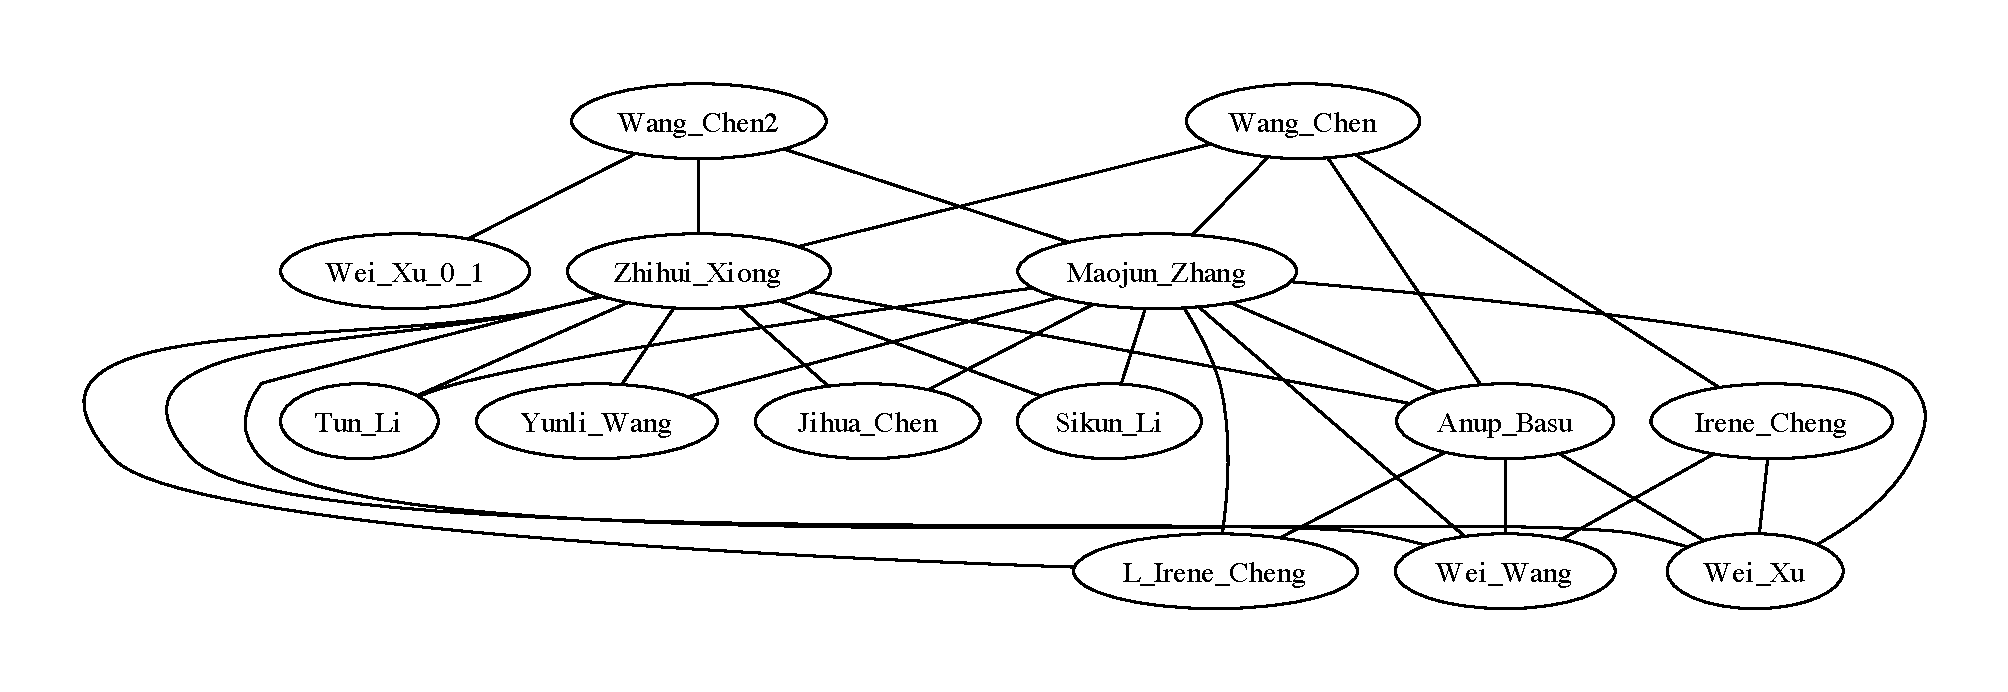
\includegraphics[width=\textwidth]{g5}
\caption{Two Wang Chen mentions (Wang Chen and Wang Chen2) are shown to be highly connected, with a connected score of 1.}
\label{fig:chen}
\end{figure*}

The venue similarity features represent how closely related the two venues are.  Intuitively, if the two venues are both in the field of machine learning, for example, International Conference on Machine Learning (ICML) and Journal of Machine Learning Research (JMLR), we would expect that a large number of authors publish in both of the venues.  Conversely, if the fields are less related, such as IEEE International Conference on Computer Communications (IEEE INFOCOM) and the journal Bioinformatics, we would expect very few authors publishing in both of them, hence an indicator that the two authors are probably different persons with the same name.

In addition, the paper ``Linking Temporal Records'' \cite{DBLP:journals/fcsc/LiDMS12} describes additional information that can be added into similarity metrics for fields. These metrics add temporal information by using the realization that over time, the fact that two fields are similar or different matters less to the task at hand. An example of such a case is affiliation information in the task of author linking in papers. Intuitively, different affiliation information for authors matters more when the papers were published close together in time in comparison to when the papers where published farther apart in time. This information is represented as the probability of the affiliation attribute changes over a time interval. The disadvantage of this approach is that labeled data is needed to learn these values.  We will also use such similarity metrics in our framework, but will be adding them as features in a CRF rather than simply using a threshold on manually weighted similarities. This should allow for better weights as well as the ability for more expressiveness in defining dependencies in our model.
% paragraph similarity_features (end)
% section methodology (end)

\section{Evaluation} % (fold)
\label{sec:evaluation}
A simple evaluation metric for our system is the accuracy
of the pairwise prediction from the CRF model.  However, it cannot
reflect the actual performance of the system.  For example, suppose
the system compares the three authors $a_1$, $a_2$, and $a_3$, and the
model predicts that $a_1$ and $a_2$ refer to the same person, $a_2$
and $a_3$ refer to the same person, but $a_2$ and $a_3$ refer to
different people.  The accuracy score would be $2/3$.  However,
computing the transitive closure corrects the wrong classification
prediction.

The author linkage problem is, at its core, a partition of the author
mentions into clusters, whose members all refer to the same person.
The coreference resolution problem in natural language processing has
the same character in which textual mentions of real world entities in
documents are clustered into groups that all refer to the same entity.
The community has developed several evaluation metrics that overcome
the problem described above.  These metrics measure how different the
true and predicted partitions are.

We evaluated our system's performance with two metrics from the
coreference resolution community.  The first is the MUC score
\cite{Vilain95} developed for a coreference resolution shared task.
This metric considers the minimal number of missing ``links'' between
author mentions required to group a set of authors together.

The other metric that we used is the $B^3$ score \cite{Bagga98b}.
This metric addresses two shortcomings of the MUC score.  MUC score
does not give any credit for separating out singletons (author
entities that no other mentions refer to), and it treats different
errors indiscriminately (merging two large partitions is equally
penalized as merging smaller partitions).

Evaluating the system on these two metrics provides a balanced view of
the performance.  The MUC score tends to favor larger clusters while
the $B^3$ gives higher penalty to such behavior.  Publications on the
coreference resolution also present multiple scores for this reason.
% section evaluation (end)

\section{Experiments} % (fold)
\label{sec:experiments}
\subsection{Baseline} % (fold)
\label{sub:baseline}
Here we compare the results of setting all classifier values to false and true. Table \ref{tab:alltrue} shows the results for all true classifications. By setting the classifier to all true, every block is classified to be in the same cluster. This results in a perfect recall, as all publications that should be clustered together are. The much worse score for B3 compared to MUC speaks to the superiority of B3 as a metric. All false results are available in table \ref{tab:allfalse}. Here the precision is perfect, since every publication is clustered into a singular cluster, thus no two publication that should not be clustered are clustered.

\begin{table}[ht]
\centering
\begin{tabular}{l || l | r r r}
 & & Precision & Recall & F1 \\ \hline
Training & B3 & 6.812 & 100.000 & 12.755 \\
 & MUC & 75.743 & 100.000 & 86.198 \\ \hline
Testing & B3 & 6.730 & 100.000 & 12.612 \\
 & MUC & 70.440 & 100.000 & 82.657 \\
\end{tabular}
\caption{All classifier predictions set to all true}
\label{tab:alltrue}
\end{table}

\begin{table}[ht]
\centering
\begin{tabular}{l || l | r r r}
 & & Precision & Recall & F1 \\ \hline
Training & B3 & 100.000 & 24.493 & 39.348 \\
 & MUC & 100.000 & 0.000 & 0.000\\ \hline
Testing & B3 & 100.000 & 29.890 & 46.024 \\
 & MUC & 100.000 & 0.000 & 0.000 \\
\end{tabular}
\caption{All classifier predictions set to all false}
\label{tab:allfalse}
\end{table}

In order to determine the contribution of each feature, we ran the classifier using only a subset of the features. Title features ended up being too sparse to have any contribution, and as such are left out of the discussion. Temporal features also did not have any additional contribution when added in. This effect is probably due to the small dataset used for training, as such statistics would be sparse in a small dataset setting.

% subsection baseline (end)
\subsection{Feature Contribution} % (fold)
\label{sub:feature_contribution}
\paragraph{Affiliation Feature} % (fold)
\label{par:affiliation_feature}
The affiliation feature set contains three discrete features. One for exact matching of the string, above a Jaro-Winker TFIDF threshold, and below the threshold. To see the advantages of using not exact string matching, we also compared just the exact string match feature to the complete feature set. The results for affiliation with just exact matchings are in table \ref{tab:exact}, and with non-exact string matching in \ref{tab:aff}. Using non-exact string matching here improves B3 by a large margin. This is because affiliation as extracted does not always have the same format, even when referring to the same institution.

\begin{table}[ht]
\centering
\begin{tabular}{l || l | r r r}
 & & Precision & Recall & F1 \\ \hline
Training & B3 & 99.324 & 71.957 & 83.454 \\
 & MUC & 99.176 & 74.587 & 85.142\\ \hline
Testing & B3 & 98.649 & 58.569 & 73.500 \\
 & MUC & 92.308 & 32.432 & 48.000 \\
\end{tabular}
\caption{Affiliation Just Exact}
\label{tab:exact}
\end{table}

\begin{table}[ht]
\centering
\begin{tabular}{l || l | r r r}
 & & Precision & Recall & F1 \\ \hline
Training & B3 & 98.398 & 79.439 & 87.908 \\
 & MUC & 98.100 & 85.331 & 91.271\\ \hline
Testing & B3 & 100.000 & 69.380 & 81.922 \\
 & MUC & 100.000 & 56.757 & 72.414 \\
\end{tabular}
\caption{Affiliation feature contribution}
\label{tab:aff}
\end{table}

% paragraph affiliation_feature (end)

\paragraph{Venue Feature} % (fold)
\label{par:venue}
The venue feature indicates the probability that for any given author, he/she publishes in both venues.  This feature serves as a proxy to how compatible two venues are, as the more authors publish in the two venues, the more related they are.  We collected the statistics from DBLP of the number of authors that published in each pair of venues that appear in our dataset.  Figure \ref{fig:venue} shows the number of venue pairs that a particular number of authors published in.  The results using only this features is shown in Table \ref{tab:venue}.  The performance is not as good as we expected.  This is possibly in part because although our general intuition that people are less likely to publish in different fields is true, the fact that ambiguous authors in DBLP skew the distribution of our statistics.  The distribution of the this feature value for the positive and negative examples in our dataset are also quite similar is another reason that this feature was not powerful.  Figure \ref{fig:venuedataset} shows the distributions of the frequencies of venue pairs for both the positive and negative pairs in our dataset.  Note that since the ratio of negative examples to positive examples is over 23 in our dataset, there is much variance in the distribution for the true examples.
\begin{figure}
  \centering
  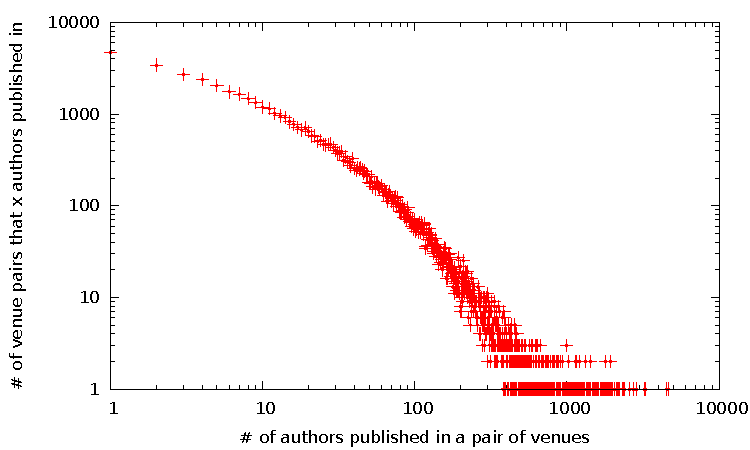
\includegraphics[width=\columnwidth]{venuepair}
  \caption{Venue Similarity.  The X axis show the number of authors published in a venue pair.  The Y axis is the total number of such venue pairs.}
  \label{fig:venue}
\end{figure}

\begin{table}
\begin{tabular}{l || l | r r r}
 & & Precision & Recall & F1 \\ \hline
Training & B3 & 41.412 & 62.659 & 49.867 \\
 & MUC & 74.561 & 70.248 & 72.340\\ \hline
Testing & B3 & 94.595 & 65.701 & 77.544 \\
 & MUC & 83.333 & 54.054 & 65.574 \\
\end{tabular}
\caption{Venue feature contribution}
\label{tab:venue}
\end{table}

\begin{figure}
  \centering
  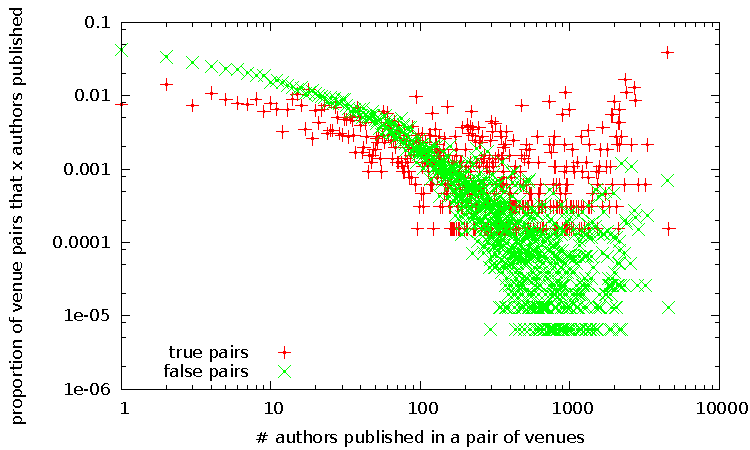
\includegraphics[width=\columnwidth]{venuestat_dataset}
  \caption{Caption}
  \label{fig:venuedataset}
\end{figure}
% paragraph venue (end)

\paragraph{Coauthor feature} % (fold)
\label{par:coauthor_feature}
The coauthor feature is one that is reliable for determining if there exists a matched author, but unreliable for determining if the authors do not match. It is often the case that our assumption is true and authors are likely to publish with in groups that are highly connected. This trend is so strong, that upon finding a publication pair with a high connected score that was marked as not the same person, it turned out to be an annotation error. However, our assumption can often fail, as many times people coauthor with somebody disjointed from their immediate research community, for example in interdisciplinary research, or when advisers publish a small number of papers with one of their students. This makes the coauthor feature a high precision, but low recall one. This trend can be seen in the two histograms in figure \ref{fig:3figs}. The histogram over pairs that are matched has many perfect connected scores whereas in the false case, there are almost none. 

Coauthor feature contribution can be seen in Table \ref{tab:coauthor}. Coauthor features seem to work well on our testing set, but have low results on our training set. This may be due to large block sizes in our training set because of the large amounts of papers whose authors have the same exact name, which will affect the transitive closure, since one false matching can merge a large amount of authors. Working on better blocking methods for cases with identical names and smarter methods than a simple transitive closure, should help our training performance.


\begin{table}[ht]
\centering
\begin{tabular}{l || l | r r r}
 & & Precision & Recall & F1 \\ \hline
Training & B3 & 41.985 & 85.405 & 56.295 \\
 & MUC & 82.946 & 88.430 & 85.600\\ \hline
Testing & B3 & 95.413 & 91.892 & 93.619 \\
 & MUC & 93.939 & 83.784 & 88.571 \\
\end{tabular}
\caption{Coauthor feature contribution}
\label{tab:coauthor}
\end{table}


\begin{figure}[ht!]%
\centering 
\subfigure[True Pairs.]{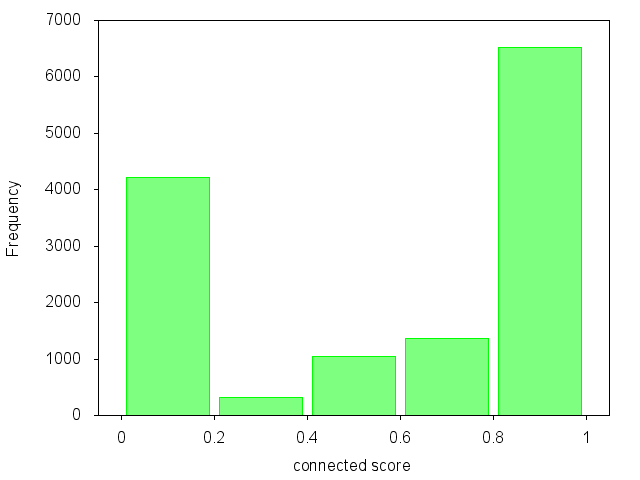
\includegraphics[scale=0.3]{trueHistogram.png}
}\qquad 
\subfigure[False Pairs.]{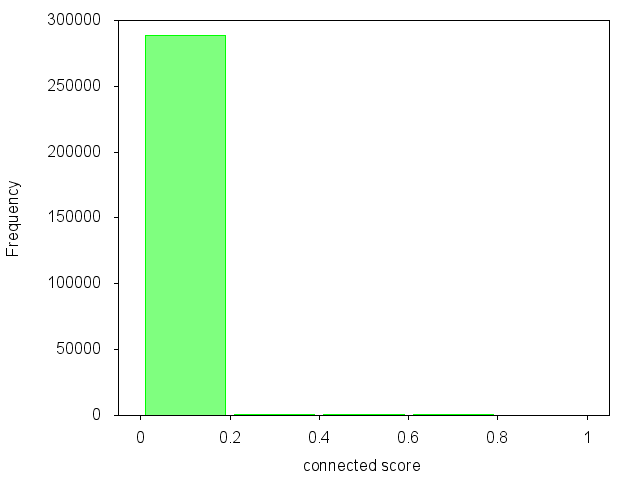
\includegraphics[scale=0.3]{falseHistogram.png}
}\\ 
\caption{Histograms for connected feature.} 
\label{fig:3figs}
\end{figure}
% paragraph coauthor_feature (end)
% subsection feature_contribution (end)

\subsection{Final Evaluation} % (fold)
\label{sub:final_evaluation}
Table \ref{tab:all} contains evaluation with all features enabled. Since venue features were weak, we evaluated also with only affiliation and coauthor features, which can be seen in table \ref{tab:some}. Again, the training results are very low, and better blocking methods should improve the results. 

\begin{table}[ht]
\centering
\begin{tabular}{l || l | r r r}
 & & Precision & Recall & F1 \\ \hline
Training & B3 & 18.307 & 97.381 & 30.820 \\
 & MUC & 79.000 & 97.934 & 87.454\\ \hline
Testing & B3 & 85.818 & 96.622 & 90.900 \\
 & MUC & 85.366 & 94.595 & 89.744 \\
\end{tabular}
\caption{Final evaluation with venue}
\label{tab:all}
\end{table}

\begin{table}[ht]
\centering
\begin{tabular}{l || l | r r r}
 & & Precision & Recall & F1 \\ \hline
Training & B3 & 37.675 & 92.109 & 53.476 \\
 & MUC & 83.729 & 94.628 & 88.846\\ \hline
Testing & B3 & 95.413 & 95.270 & 95.341\\
 & MUC & 94.444 & 91.892 & 93.151 \\
\end{tabular}
\caption{Final evaluation with only affiliation and coauthor}
\label{tab:some}
\end{table}

% subsection final_evaluation (end)
% section experiments (end)


\bibliographystyle{plain}
\bibliography{refs}
\end{document}
